%!TEX root = ../DSGEnotes.tex
\section{有限元}
\label{sec:finele}

第\ref{sec:variational-bvp}节介绍了如何将边界积分问题转换为变分问题,本节进一步介绍求得变分问题近似解的方法。首先介绍如何设定合适的有限维检测空间,然后证明索伯列夫空间的一些近似特性。出于简化的考虑,在这里我们只考虑用低阶多项式来构建基方程;更一般形式的有限元近似方法,可参考 \cite{Cheng:2005cd,Brenner:2008hf}。

\subsection{参考元}
\label{sec:finele-reference-elements}
设一个有界域$\Omega \subset \mathbb{R}^{d}, d=1,2,3$,域的边界可能是多边形(polygonal, $d=2$)或多面体(polyhedra, $d=3$)。将某一个$\overline{\Omega}$分解为含有有限个网格(mesh)\index{mesh \dotfill 网格} $\tau_{\ell}$的序列$\left\{ \mathcal{T}_{N} \right\}_{N \in \mathbb{N}}$,分解(decomposition)\index{decomposition! \dotfill 分解(有限元)}可写作
\begin{equation}
  \label{eq:finele-ref-decomposition}
  \overline{\Omega} = \overline{\mathcal{T}_{N}} = \bigcup_{\ell = 1}^{N} \overline{\tau}_{\ell}.
\end{equation}

\subsubsection{基本概念}
在最简单的例子中,每一个网格对应一个区间(interval, $d=1$),三角形(triangle, $d=2$),或多面体(tetrahedron, $d=3$)。$\mathcal{T}_{N}$中全部结点(nodes)\index{node \dotfill 结点}的集合用$\left\{ x_{k} \right\}_{k=1}^{M}$来表示。对于$d=2,3$的情况,边(edge)\index{edge \dotfill 边}用$\left\{ k_{j} \right\}_{j=1}^{K}$来表示。分解$\tau_{\ell}$和对应结点$x_{k}$的关系,可参考图\ref{fig:finele-ref-element-nodes}
。

\begin{figure}[htbp]
  \centering
  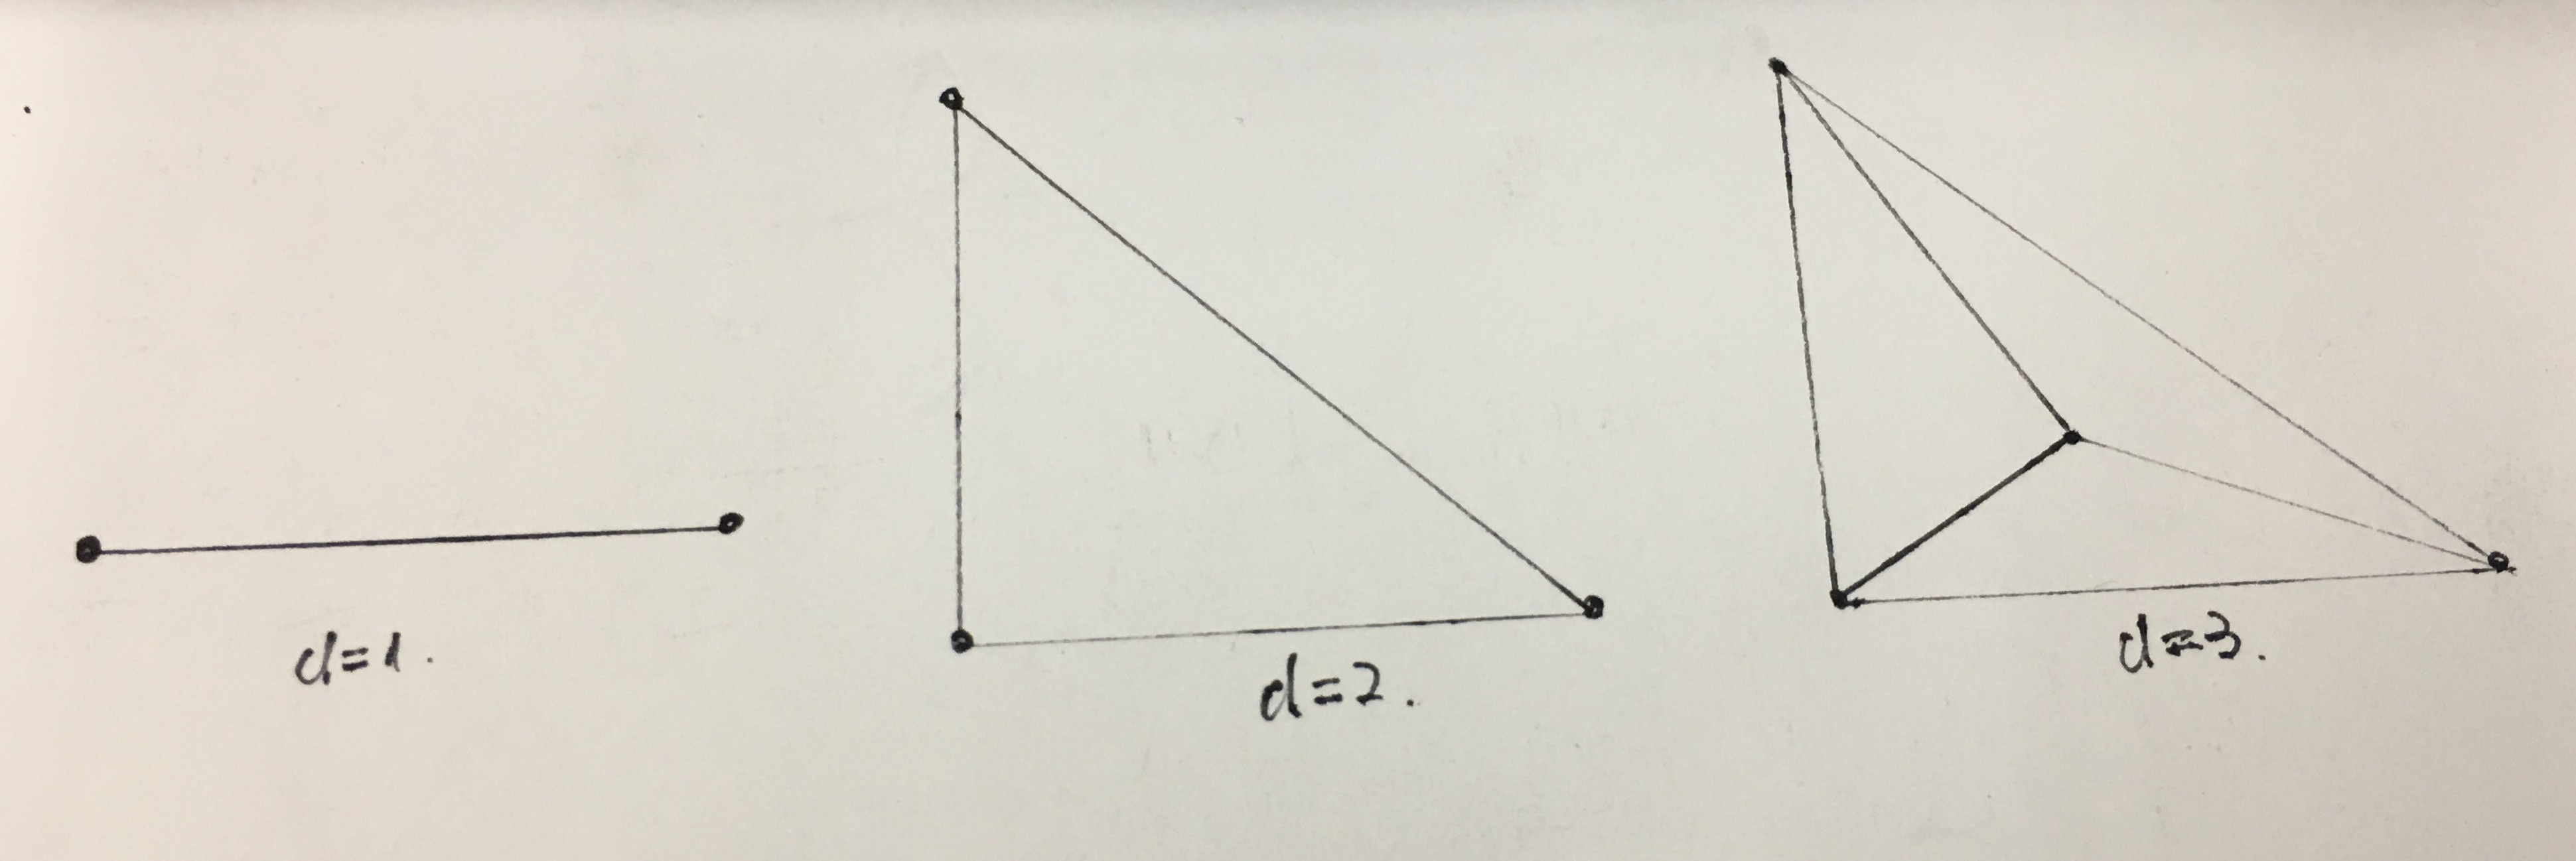
\includegraphics[width=4in]{./figures/20171209-finele-nodes}
 \caption{有限元$\tau_{\ell}$及其结点$x_{k}$}
\label{fig:finele-ref-element-nodes}

%  \small{注:实线表示名义资金流动。虚线表示实际物质流动。}
\end{figure}

定义以下三个集合
\begin{itemize}
  \item $I(k)$表示全部网格$\tau_{\ell}$的集合
  \begin{equation*}
    I(k) \coloneqq \left\{ \ell \in \mathbb{N}: x_{k} \in \overline{\tau}_{\ell} \right\}, \quad k = 1, \ldots, M,
  \end{equation*}
  \item $J(\ell)$表示网格$\overline{\tau}_{\ell}$中全部结点$x_{k}$的集合
  \begin{equation*}
    J(\ell) \coloneqq \left\{ k \in \mathbb{N}: x_{k} \in \overline{\tau}_{\ell} \right\}, \quad \ell = 1, \ldots, N,
  \end{equation*}
  可见$\dim J(\ell) = d+1$,
  \item $K(j)$表示网格$\overline{\tau}_{\ell}$中全部边$k_{j}$的集合
  \begin{equation*}
    K(j) \coloneqq \left\{ \ell \in \mathbb{N} : k_{j} \in \overline{\tau}_{\ell} \right\}, \quad j = 1, \ldots, K.
  \end{equation*}
\end{itemize}

如果有限元分解\eqref{eq:finele-ref-decomposition}中,所有两个相邻元之间都有共享的结点(d=1,2,3),边(d=2,3),三角形(d=3),那么我们称这种分解为容许分解(admissible decomposition)\index{decomposition!admissible \dotfill 容许分解}。以$d=2$为例,容许和不容许分解的例子见图\ref{fig:finele-ref-decomp-admissible-example}。
\begin{figure}[htbp]
  \centering
  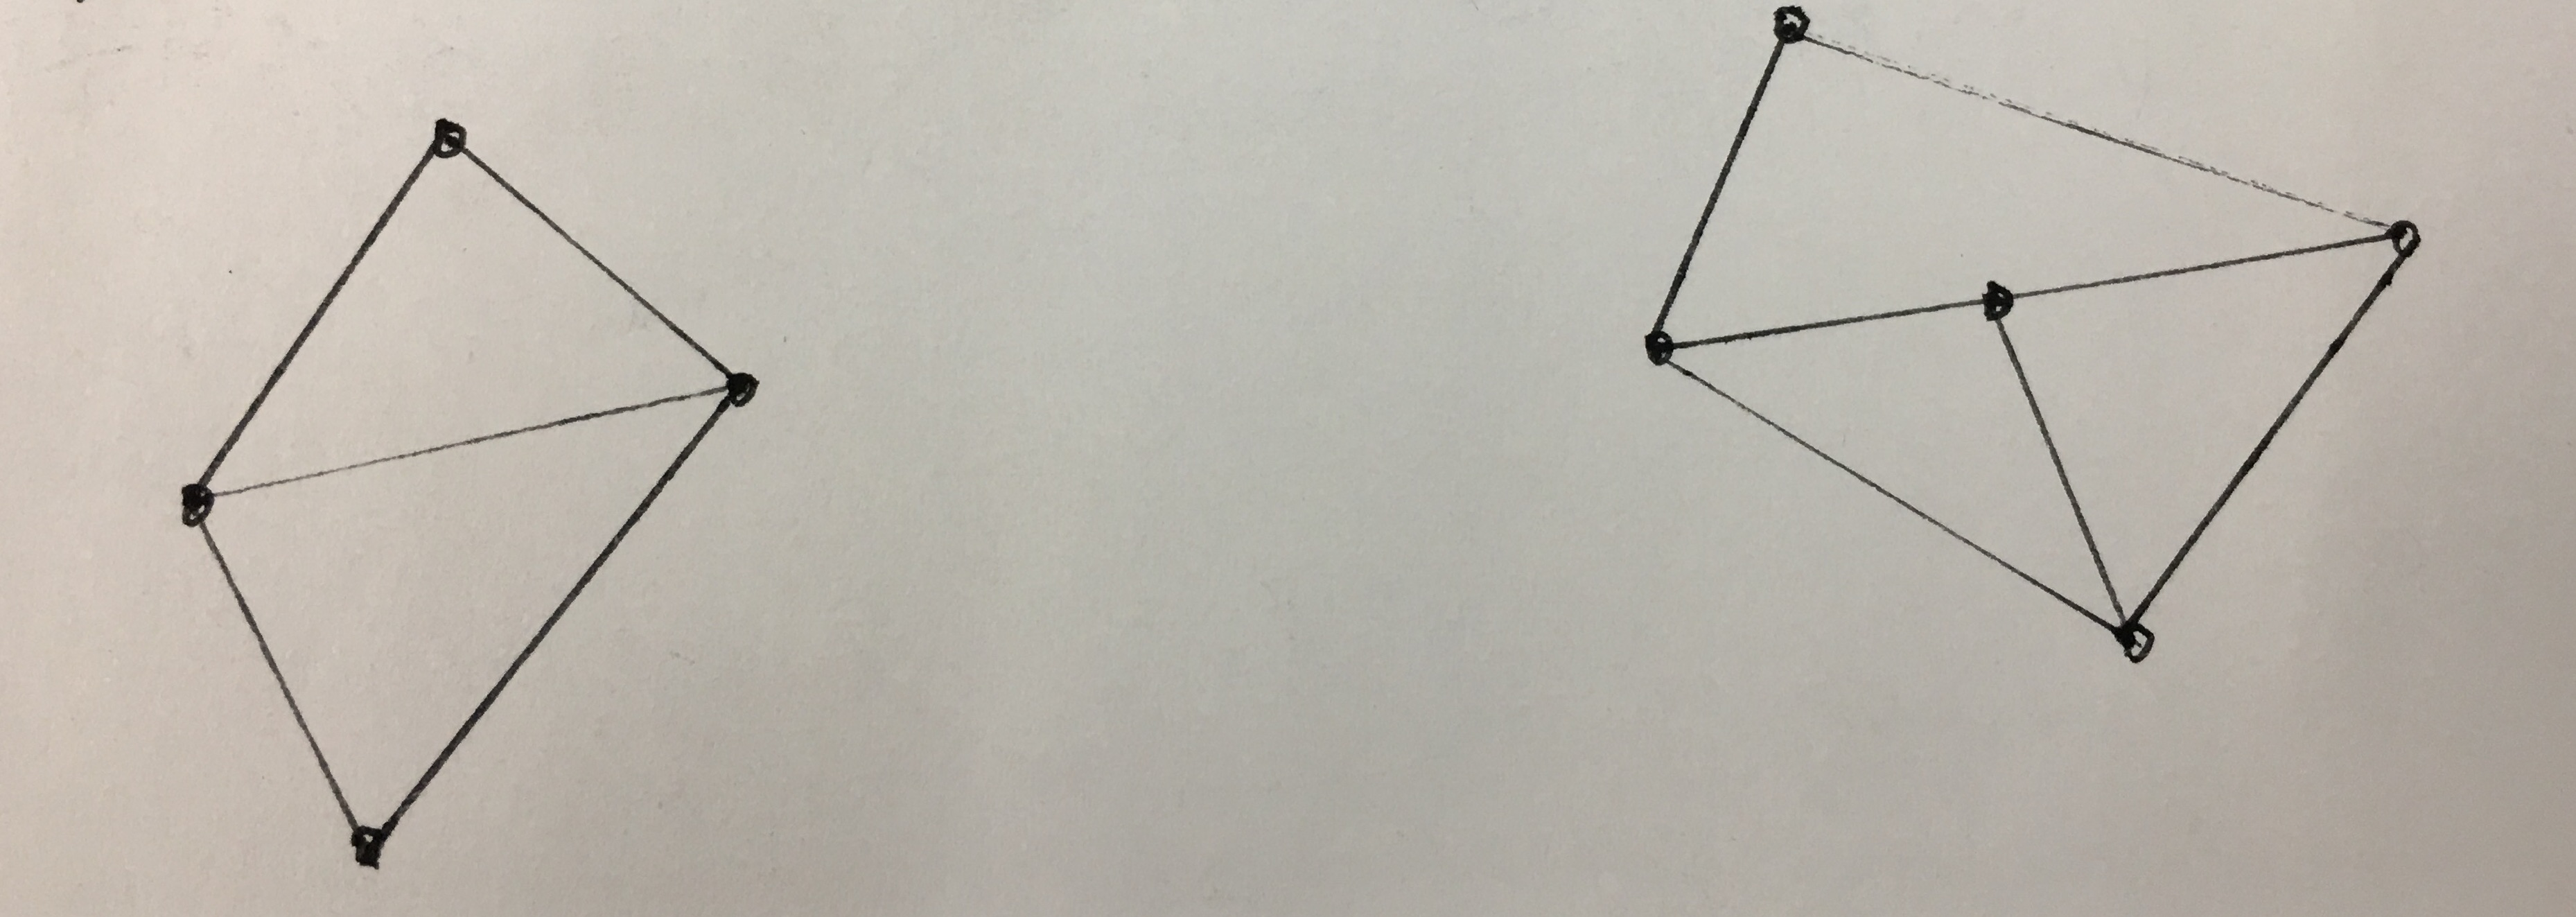
\includegraphics[width=4in]{./figures/20171209-decompo-adm-inadm.jpg}
 \caption{容许分解,以及不容许分解的三角分解($d=2$)}
\label{fig:finele-ref-decomp-admissible-example}

%  \small{注:实线表示名义资金流动。虚线表示实际物质流动。}
\end{figure}

在这里我们只考虑可计算域$\Omega$中容许分解的情况。对于某一有限元$\tau_{\ell}$,作如下定义
\begin{itemize}
  \item $\Delta_{\ell}$表示体积(volume)
  \begin{equation*}
    \Delta_{\ell} \coloneqq \int_{\tau_{\ell}} dx,
  \end{equation*}
  \item $h_{\ell}$表示局部网格尺寸(local mesh size)\index{mesh size!local \dotfill 局部网格尺寸}
  \begin{equation*}
    h_{\ell} \coloneqq \Delta_{\ell}^{\frac{1}{d}},
  \end{equation*}
  \item $d_{\ell}$表示(最大)直径,即有限元$\tau_{\ell}$中最长的一条边的长度
  \begin{equation*}
    d_{\ell} \coloneqq \sup_{x,y \in \tau_{\ell}}
    \left| x - y \right|,
  \end{equation*}
  显然对于$d=1$,我们有$\Delta_{\ell} = h_{\ell} = d_{\ell}$,
  \item 对应$d_{\ell}$,$r_{\ell}$表示(可包住)有限元$\tau_{\ell}$的最大圆($d=2$)或球体($d=3$)的半径。
\end{itemize}

经容许分解\eqref{eq:finele-ref-decomposition}后得到的有限元$\tau_{\ell}$,如果直径$d_{\ell}$由半径$r_{\ell}$约束而一致有界(uniformly bounded),即满足
\begin{equation*}
  d_{\ell} \le c_{F} \, r_{\ell}, \quad \ell = 1,\ldots,N,
\end{equation*}
那么我们称$\tau_{\ell}$为正则型有限元(regular finite element)\index{finite element!regular \dotfill 正则型有限元},其中常数$c_{F}$与$\mathcal{T}_{N}$:
\begin{itemize}
  \item 对于$d=2$的情况
  \begin{equation*}
    \begin{split}
      &\pi r_{\ell}^{2} \le \Delta_{\ell} = h_{\ell}^{2} \le d_{\ell}^{2} \le c_{F}^{2} r_{\ell}^{2}, \\
      \hookrightarrow &\pi^{\frac{1}{2}} r_{\ell} \le h_{\ell} \le d_{\ell} \le c_{F} r_{\ell},
    \end{split}
  \end{equation*}
  \item 对于$d=3$的情况
  \begin{equation*}
    \begin{split}
      &\frac{4}{3} \pi r_{\ell}^{3} \le \Delta_{\ell} = h_{\ell}^{3} \le d_{\ell}^{3} = c_{F}^{3} r_{\ell}^{3}, \\
      \hookrightarrow & \left( \frac{4}{3} \pi \right)^{\frac{1}{3}}
      r_{\ell} \le h_{\ell} \le d_{\ell} \le c_{F} r_{\ell}.
    \end{split}
  \end{equation*}
\end{itemize}

我们将最大、最小的局部网格尺寸分别定义为$h_{\max},h_{\min}$
\begin{equation*}
  \begin{split}
    h_{\max} & \coloneqq \max_{\ell =1,\ldots,N} h_{\ell}, \\
    h_{\min} & \coloneqq \min_{\ell =1,\ldots,N} h_{\ell},
  \end{split}
\end{equation*}
对应地将全局网格尺寸(global mesh size)\index{mesh size!global \dotfill 全局网格尺寸}定义为
\begin{equation*}
  h = h_{\max}.
\end{equation*}

如果$h_{\max}$和$h_{\min}$的比值小于等于一个全常数$c_{G} \ge 0$,即以下比值有界
\begin{equation*}
  \frac{h_{\max}}{h_{\min}} \le c_{G},
\end{equation*}
那么我们称对应的分解$\mathcal{T}_{N}$是全局拟一致的(globally quasi-uniform)\index{quansi-uniform!globally \dotfill 全局拟一致}的;$c_{G} \ge 1$的值与$N \in \mathbb{N}$无关。

对应地,如果对于任何两个临近的有限元$\tau_{\ell}$和$\tau{j}$都有
\begin{equation*}
  \frac{h_{\ell}}{h_{j}} \le c_{L}, \ell,j = 1,\ldots,N,
\end{equation*}
那么我们称这样的分解$\mathcal{T}_{N}$为局部拟一致(locally quasi-uniform)\index{quasi-uniform!locally \dotfill 局部拟一致}。
对于某一组相邻的有限元$\overline{\tau}_{\ell}$和$\overline{\tau}_{j}$,如果$\overline{\tau}_{\ell} \cap \overline{\tau}_{j}$包括不少于1个结点、1条边或1个三角形,那么我们称二者为相邻有限元(neighboring)\index{finite element!neighboring \dotfill 相邻有限元}。

\subsubsection{一维空间的局部参数化}
$d=1$时,每个有限元$\tau_{\ell}$都可以用局部参数化(local parameterization)\index{parameterization!local \dotfill 局部参数化}的形式予以描述。尤其是对于$x \in \tau_{\ell}, \, \ell_{1}, \ell_{2} \in J(\ell)$,我们有
\begin{equation*}
  x = x_{\ell_{1}} + \xi \left( x_{\ell_{2}} - x_{\ell_{1}} \right)
  =x_{\ell_{1}} + \xi h_{\ell}, \quad \xi \in (0,1),
\end{equation*}
其中我们将$\tau \coloneqq (0,1)$称为参考元(reference element)\index{reference element \dotfill 参考元}。

考虑这样一个方程$\nu(x), \, x \in \tau_{\ell}$,由上面的定义可得
\begin{equation*}
  \nu(x) = \nu(x_{\ell_{1}} + \xi h_{\ell} ) \eqqcolon \widetilde{\nu}_{\ell}(\xi), \quad \forall \, \xi \in \tau,
\end{equation*}
即对于$x \in \tau_{\ell}$,我们可以将方程$\nu(x)$识别为参考元中的方程$\widetilde{\nu}_{\ell}(\xi), \, \xi \in \tau$,对应范数

\begin{equation*}
  \begin{split}
    \left\| \nu \right\|_{L^{2}(\tau_{\ell})}^2
    &= \int_{\tau_{\ell}} \left( \nu(x) \right)^{2} \, dx = \int_{\tau} \left| \widetilde{\nu}_{\ell}(\xi) \right|^{2} h_{\ell} \, d \xi \\
    & = h_{\ell} \left\| \widetilde{\nu}_{\ell}(\xi) \right\|_{L^{2}(\tau)}^{2}.
  \end{split}
\end{equation*}

我们经常需要计算识别方程的导数,根据链式法则\eqref{eq:chain-rule-exa}可得
\begin{enumerate}
  \item 一阶导数
  \begin{equation*}
    \begin{split}
      &\frac{d}{d \xi} \widetilde{\nu}_{\ell}(\xi) = h_{\ell} \frac{d}{d x} \nu(x), \\
      \hookrightarrow & \frac{d}{d x}\nu(x) =
      h_{\ell}^{-1} \frac{d}{d \xi} \widetilde{\nu}_{\ell}(\xi), \quad \, x \in \tau_{\ell}, \, \xi \in \tau.
    \end{split}
  \end{equation*}
  \item 推广至高阶导数如$m \in \mathbb{N}$的情况
  \begin{equation*}
    \begin{split}
      \frac{d^{m}}{d x^{m}} \nu(x) = h^{- m} \frac{d^{m}}{d \xi^{m}}
      \widetilde{\nu}_{\ell}(\xi), \quad \, x \in \tau_{\ell}, \, \xi \in \tau,
    \end{split}
  \end{equation*}
  对应局部范数
  \begin{equation}
    \label{eq:finele-ref-local-norm}
    \left\|
    \frac{d^{m}}{d x^{m}}  \nu
    \right\|_{L^{2}(\tau_{\ell})}^{2}
    = h_{\ell}^{1-2m}
    \left\|
    \frac{d^{m}}{d \xi^{m}} \widetilde{\nu}_{\ell}
    \right\|_{L^{2}(\tau)}^{2}, \quad m \in \mathbb{N}_{0}.
  \end{equation}
\end{enumerate}

\subsubsection{二维空间的局部参数化}
$d=2$时,有限元$\tau_{\ell}$和参考元$\tau$的关系,见图\ref{fig:finele-ref-finele-refele}。

\begin{figure}[htbp]
  \centering
  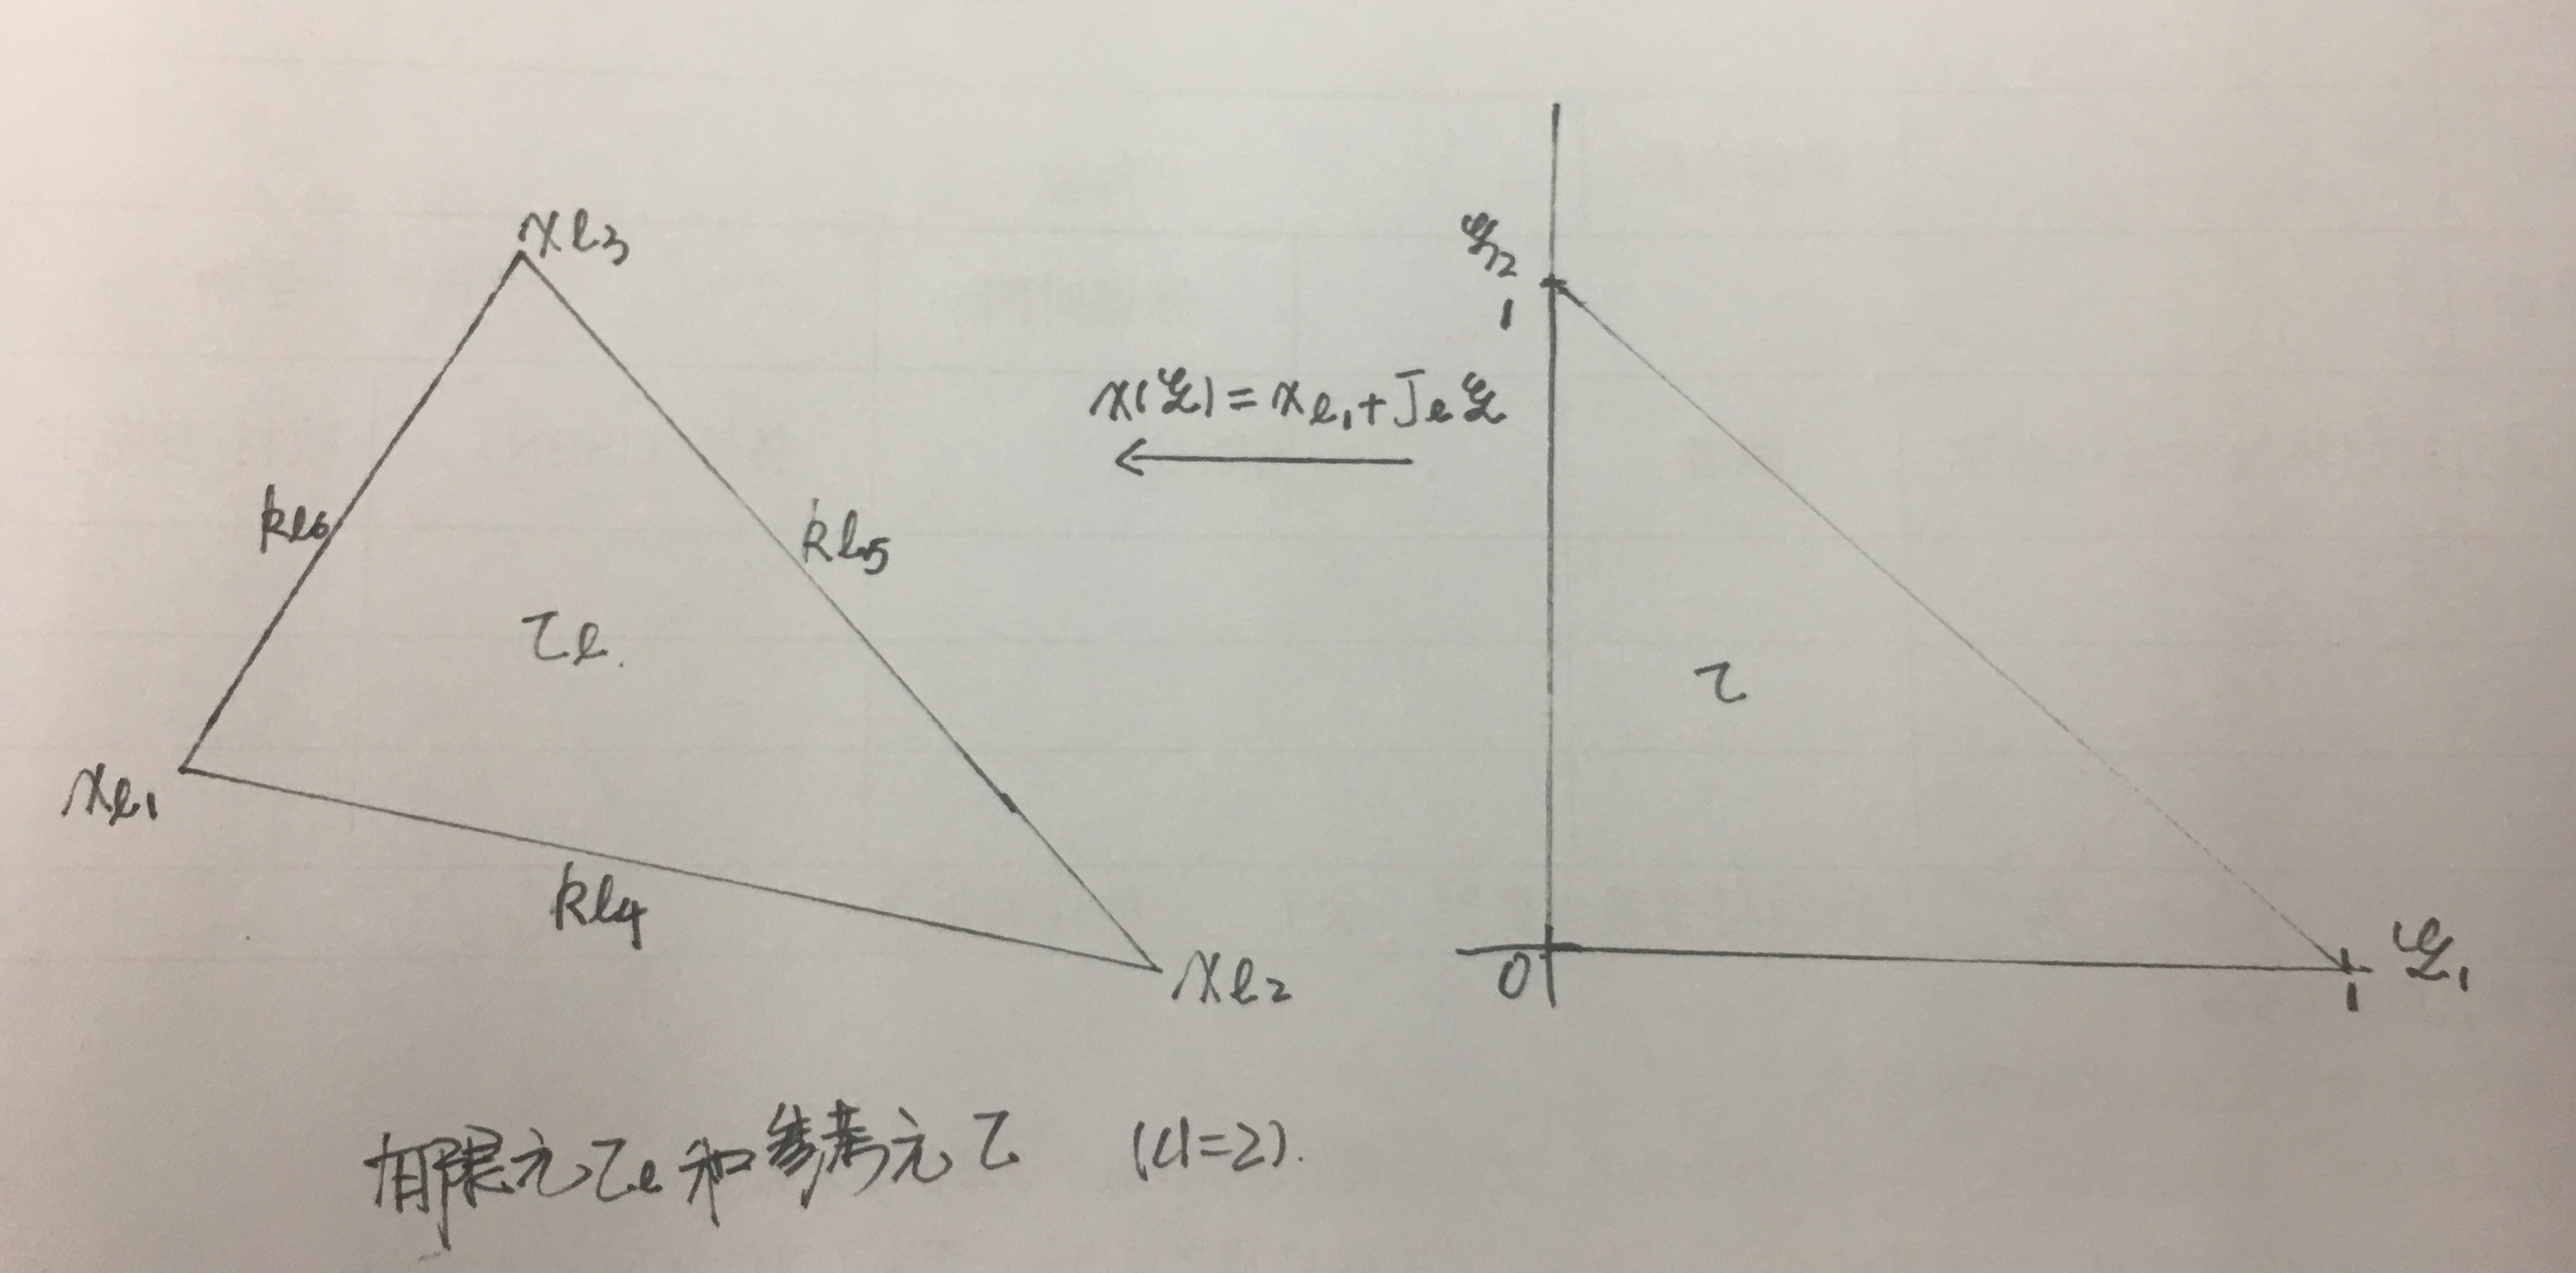
\includegraphics[width=4in]{./figures/20171210-finele-refele}
 \caption{有限元$\tau_{\ell}$和参考元$\tau$($d=2$)}
\label{fig:finele-ref-finele-refele}

%  \small{注:实线表示名义资金流动。虚线表示实际物质流动。}
\end{figure}

参考元$\tau$由下面三角形给出
\begin{equation}
  \label{eq:finele-ref-d2-refele-def}
  \tau = \left\{
  \xi \in \mathbb{R}^{2}: 0 \le \xi_{1} \le 1, \, 0 \le \xi_{2} \le 1 - \xi_{1} \right\}.
\end{equation}

对$x \in \tau_{\ell}$作局部参数化
\begin{equation*}
  x = x_{\ell_{1}} + \sum_{i=1}^{2} \xi_{i} \left( x_{\ell_{i+1}} - x_{\ell_{1}} \right) = x_{\ell_{1}} + J_{\ell} \, \xi, \quad \xi \in \tau,
\end{equation*}
其中$J_{\ell}$是个雅各比矩阵
\begin{equation*}
  J_{\ell} \coloneqq
  \begin{pmatrix}
    x_{\ell_{2}, 1} - x_{\ell_{1}, 1} &
    x_{\ell_{3}, 1} - x_{\ell_{1}, 1} \\
    x_{\ell_{2}, 2} - x_{\ell_{1}, 2} &
    x_{\ell_{3}, 2} - x_{\ell_{1}, 2}
  \end{pmatrix}.
\end{equation*}

由此我们得有限元$\tau_{\ell}$的面积,同时也是体积
\begin{equation*}
\begin{split}
    \Delta_{\ell} & = \int_{\tau_{\ell}} d s_{x} = \int_{\tau} \left| \det J_{\ell} \right| d \xi \\
    & = \left| \det J_{\ell} \right| \int_{0}^{1} \int_{0}^{1-\xi_{1}} d \xi_{2} d \xi_{1} = \frac{1}{2} \left| \det J_{\ell} \right|,
\end{split}
\end{equation*}
\begin{equation}
  \label{eq:finele-ref-d2-volume-matrix-determinant}
  \hookrightarrow \left| \det J_{\ell} \right| = 2 \Delta_{\ell}.
\end{equation}

$\nu(x), \, x \in \tau_{\ell}$对应的识别方程可表示为
\begin{equation*}
  \nu(x) = \nu \left( x_{\ell_{1}} + J_{\ell} \xi \right)
  \eqqcolon \widetilde{\nu}_{\ell}(\xi), \quad \xi \in \tau.
\end{equation*}

继续应用链式法则
\begin{equation*}
  \begin{split}
    & \triangledown_{\xi} \widetilde{\nu}_{\ell}(\xi) = J_{\ell}^{\top} \triangledown_{x} \nu(x), \\
    \hookrightarrow & \triangledown_{x} \nu(x) = J_{\ell}^{- \top} \triangledown_{\xi} \widetilde{\nu}_{\ell}(\xi).
\end{split}
\end{equation*}

等价范数的测度由下引理给出。
\begin{lemma}[识别方程等价范的测度($d=2$)]
  \label{lemma:finele-ref-d2-norm-equiv}
  $d=2, \, m \in \mathbb{N}_{0}$的情况下,识别方程的等价范满足不等式关系
  \begin{equation}
    \label{eq:finele-ref-d2-norm-equiv}
    \begin{split}
      \frac{1}{c_{m}} \left( 2 \Delta_{\ell} \right)^{1-m} \,
      \left\| \triangledown_{\xi}^{m}
      \widetilde{\nu}_{\ell}
      \right\|_{L^{2}(\tau)}^{2}
      \le \left\| \triangledown_{x}^{m} \nu \right\|_{L^{2}(\tau_{\ell})}^{2}
      \le c_{m} \, \left( 2 \Delta_{\ell} \right)^{1-m} \,
      \left\| \triangledown_{\xi}^{m} \widetilde{\nu}_{\ell}
      \right\|_{L^{2}(\tau)}^{2},
    \end{split}
  \end{equation}
  其中常数$c_{m} = \left( \frac{c_{F}^{2}}{\pi} \right)^{m}$。
\end{lemma}

\begin{proof}
  对于$m \in \mathbb{N}_{0}$,分三种情况来分别证明。
\begin{enumerate}
  \item $m=0$时。
  \begin{equation*}
    \begin{split}
      \left\| \nu \right\|_{L^{2}(\tau_{\ell})}^{2}
      &= \int_{\tau_{\ell}} \left| \nu(x) \right|^{2} \, dx \\
      & = \int_{\tau} \left| \widetilde{\nu}_{\ell} (\xi) \right|^{2}
      \left| \det J_{\ell} \right| \, d \xi \\
      & = 2 \Delta_{\ell} \, \left\| \widetilde{\nu}_{\ell} (\xi) \right\|_{L^{2}(\tau)}^{2},
    \end{split}
  \end{equation*}
  可证得\eqref{eq:finele-ref-d2-norm-equiv}成立。

  \item $m=1$时。
  \begin{equation*}
    \begin{split}
      \left\| \triangledown_{x} \nu \right\|_{L^{2}(\tau_{\ell})}^2
      & = \int_{\tau_{\ell}} \left| \triangledown_{x} \nu(x) \right|^{2} \, dx \\
      & = \int_{\tau}
      \left| J_{\ell}^{- \top} \triangledown_{\xi} \widetilde{\nu}_{\ell} (\xi) \right|^{2} \,
      \left| \det J_{\ell} \right|
      \, d \xi\\
      & = 2 \Delta_{\ell} \int_{\tau}
      \left(
      J_{\ell}^{-\top} \triangledown_{\xi} \widetilde{\nu}_{\ell} (\xi),
      \triangledown_{\xi} \widetilde{\nu}_{\ell} (\xi)
      \right) \,
      d \xi \\
      & = 2 \Delta_{\ell} \int_{\tau}
      \left(
      J_{\ell}^{-1} J_{\ell}^{-\top} \triangledown_{\xi} \widetilde{\nu}_{\ell} (\xi),
      \triangledown_{\xi} \widetilde{\nu}_{\ell} (\xi)
      \right) \, d \xi \\
      & \le 2 \Delta_{\ell} \lambda_{\max} \left(J_{\ell}^{-1} J_{\ell}^{-\top} \right) \,
      \int_{\tau}
      \left|
      \triangledown_{\xi} \widetilde{\nu}_{\ell} (\xi)
      \right| \, d_{\xi} \\
      & = 2 \Delta_{\ell} \lambda_{\max} \left(J_{\ell}^{-1} J_{\ell}^{-\top} \right) \,
      \left\|
      \triangledown_{\xi} \widetilde{\nu}_{\ell} (\xi)
      \right\|_{L^{2}(\tau)}^{2},
    \end{split}
  \end{equation*}

  以及类似地
  \begin{equation*}
    \begin{split}
      \left\| \triangledown_{x} \nu \right\|_{L^{2}(\tau_{\ell})}^2
      \ge 2 \Delta_{\ell} \, \lambda_{\min} \left(J_{\ell}^{-1} J_{\ell}^{-\top} \right) \,
      \left\|
      \triangledown_{\xi} \widetilde{\nu}_{\ell} (\xi)
      \right\|_{L^{2}(\tau)}^{2}.
    \end{split}
  \end{equation*}

  以上两个不等式都需要计算矩阵$\left(J_{\ell}^{-1} J_{\ell}^{-\top} \right)$的特征值,这可以从$\left(J_{\ell}^{\top} J_{\ell} \right)$开始
  \begin{equation*}
    J_{\ell}^{\top} J_{\ell} =
    \begin{pmatrix}
      a^{2} & a b \cos \alpha \\
      a b \cos \alpha & b^{2}
    \end{pmatrix},
  \end{equation*}
  其中
\begin{equation*}
  \begin{split}
    a & \coloneqq \left| x_{\ell_{2}} - x_{\ell_{1}} \right|, \\
    b & \coloneqq \left| x_{\ell_{3}} - x_{\ell_{1}} \right|, \\
    \alpha  & \coloneqq \sphericalangle
    \left( x_{\ell_{3}} - x_{\ell_{1}}, x_{\ell_{2}} - x_{\ell_{1}} \right).
  \end{split}
\end{equation*}

$\left(J_{\ell}^{-1} J_{\ell}^{-\top} \right)$的特征值为\footnote{善用Mathematica!}
\begin{equation*}
  \lambda_{1,2} = \frac{1}{2}
  \left[
  a^{2} + b^{2} \pm
  \left(
  \left(a^{2} - b^{2} \right)^2
  + 4 a^{2} b^{2} \left( \cos \alpha \right)^{2}
  \right)^{\frac{1}{2}}
  \right]
\end{equation*}
\begin{itemize}
  \item 对应的上限特征值$\lambda_{1}$有
  \begin{equation*}
    \frac{1}{2} \left( a^{2} + b^{2} \right) \le \lambda_{1} \le a^{2} + b^{2},
  \end{equation*}
  \item 两个特征值的乘积,根据\eqref{eq:finele-ref-d2-volume-matrix-determinant}有
  \begin{equation*}
    \lambda_{1} \lambda_{2} = \det \left| J_{\ell}^{\top} J_{\ell} \right|
    = \det \left| J_{\ell} \right|^{2}
    = 4 \Delta_{\ell}^{2}.
  \end{equation*}
  \item 因此对应的下限特征值$\lambda_{2}$有
  \begin{equation*}
    \lambda_{2} = \frac{4 \Delta_{\ell}^{2}}{\lambda_{1}} \ge \frac{4 \Delta_{\ell}^{2}}{a^{2} + b^{2}}.
  \end{equation*}
  \item 由此我们有
  \begin{equation*}
    \frac{4 \Delta_{\ell}^{2}}{a^{2} + b^{2}}
    \le \lambda_{\min}\left( J_{\ell}^{\top} J_{\ell} \right)
    \le \lambda_{\max}\left( J_{\ell}^{\top} J_{\ell} \right)
    \le a^{2} + b^{2}.
  \end{equation*}
  \item 此外根据定义我们有
  \begin{equation*}
    a^{2} + b^{2} \le 2 d_{\ell}^{2} \le 2 c_{F}^{2} r_{\ell}^{2}
    \le \frac{2 c_{F}^{2}}{\pi} \Delta_{\ell},
  \end{equation*}
  代入上式,整理得
  \begin{equation*}
    \frac{2 \pi}{c_{F}^{2}} \Delta_{\ell}
    \le \lambda_{\min} \left( J_{\ell}^{\top} J_{\ell} \right)
    \le \lambda_{\max}\left( J_{\ell}^{\top} J_{\ell} \right)
    \le \frac{2 c_{F}^{2}}{\pi} \Delta_{\ell}.
  \end{equation*}
\end{itemize}

所以,$J_{\ell}^{\top} J_{\ell}$的逆矩阵$J_{\ell}^{-1} J_{\ell}^{-\top}$的特征值满足
\begin{equation*}
  \begin{split}
    &\frac{\pi}{c_{F}^{2}} \left( 2 \Delta_{\ell} \right)^{-1}
    \le \lambda_{\min} \left( J_{\ell}^{-1} J_{\ell}^{-\top} \right)
    \le \lambda_{\max} \left( J_{\ell}^{-1} J_{\ell}^{-\top} \right)
    \le \frac{c_{F}^{2}}{\pi} \left( 2 \Delta_{\ell} \right)^{-1}, \\
    \hookrightarrow &
    \left( \frac{1}{c_{m}} \right) \left( 2 \Delta_{\ell} \right)^{-1}  \left( 2 \Delta_{\ell} \right)^{-1}
    \le \lambda_{\min} \left( J_{\ell}^{-1} J_{\ell}^{-\top} \right)
    \le \lambda_{\max} \left( J_{\ell}^{-1} J_{\ell}^{-\top} \right)
    \le c_{m} \left( 2 \Delta_{\ell} \right)^{-1},
  \end{split}
\end{equation*}
因此证得\eqref{eq:finele-ref-d2-norm-equiv}。

\item $m>1$时,可通过递归重复上述步骤证得\eqref{eq:finele-ref-d2-norm-equiv}。
\end{enumerate}
\end{proof}

\subsubsection{三维空间的局部参数化}
$d=3$时,参考元$\tau$表现为四面体(tetraderon)形式
\begin{equation*}
  \begin{split}
    \tau = \left\{
    \xi \in \mathbb{R}^{3} :
    0 \le \xi_{1} \le 1, \,
    0 \le \xi_{2} \le 1 - \xi_{1}, \,
    0 \le \xi_{3} \le 1 - \xi_{1} - \xi_{2}
    \right\}.
  \end{split}
\end{equation*}

对$x \in \tau_{\ell}$作局部参数化
\begin{equation*}
  x = x_{\ell_{1}} + \sum_{i=1}^{3} \xi_{1} \left( x_{\ell_{i+1}} - x_{\ell_{1}} \right)
  = x_{\ell_{1}} + J_{\ell} \xi, \quad \, \xi \in \tau,
\end{equation*}
其中雅各比矩阵
\begin{equation*}
  J_{\ell} =
  \begin{pmatrix}
    x_{\ell_{2},1} - x_{\ell_{1},1} &
    x_{\ell_{3},1} - x_{\ell_{1},1} &
    x_{\ell_{4},1} - x_{\ell_{1},1} \\
    x_{\ell_{2},2} - x_{\ell_{1},2} &
    x_{\ell_{3},2} - x_{\ell_{1},2} &
    x_{\ell_{4},2} - x_{\ell_{1},2} \\
    x_{\ell_{2},3} - x_{\ell_{1},3} &
    x_{\ell_{3},3} - x_{\ell_{1},3} &
    x_{\ell_{4},3} - x_{\ell_{1},3}
  \end{pmatrix}.
\end{equation*}

有限元的体积
\begin{equation*}
  \begin{split}
  \Delta_{\ell} & = \int_{\tau_{\ell}} d s_{x}
  = \int_{\tau} \left| \det J_{\ell} \right| d \xi \\
  & = \left| \det J_{\ell} \right| \,
  \int_{0}^{1} \int_{0}^{1 - \xi_{1}} \int_{0}^{1 - \xi_{1} - \xi_{2}} \, d \xi_{3} \, d \xi_{2} \, d \xi_{1} \\
  & = \frac{1}{6} \left| \det J_{\ell} \right|,
\end{split}
\end{equation*}
\begin{equation}
  \label{eq:finele-ref-d3-volume-matrix-determinant}
  \hookrightarrow \left| \det J_{\ell} \right| = 6 \Delta_{\ell}.
\end{equation}

用识别方程$\widetilde{\nu}_{\ell}(\xi), \, \xi \in \tau$来识别$\nu(x), \, x \in \tau_{\ell}$
\begin{equation*}
  \nu(x) = \nu \left( x_{\ell_{1}} + J_{\ell} \xi \right)
  \eqqcolon \widetilde{\nu}_{\ell}(\xi), \quad \xi \in \tau.
\end{equation*}

根据链式法则,可得导数
\begin{equation*}
  \begin{split}
    & \triangledown_{\xi} \widetilde{\nu}_{\ell} (\xi) = J_{\ell}^{\top} \triangledown_{x} \nu(x), \\
    & \hookrightarrow \triangledown_{x} \nu(x) = J_{\ell}^{\top} \triangledown_{\xi} \widetilde{\nu}_{\ell} (\xi).
  \end{split}
\end{equation*}

等价范数的测度见下引理。
\begin{lemma}[识别方程等价范的测度(d=3)]
  \label{lemma:finele-ref-d3-norm-equiv}
  $d=3,\,m\in \mathbb{N}_{0}$的情况下,识别方程的等价范满足不等式关系
  \begin{equation}
    \label{eq:finele-ref-d3-norm-equiv}
    c_{1} \Delta_{\ell} h_{\ell}^{- 2 m} \,
    \left\|
    \triangledown_{\xi}^{m} \widetilde{\nu}_{\ell}
    \right\|_{L^{2}(\tau)}^{2}
    \le \left\| \triangledown_{x}^{m} \nu
    \right\|_{L^{2}(\tau_{\ell})}^{2}
    \le c_{2} \Delta_{\ell} h_{\ell}^{- 2 m}
    \left\|
    \triangledown_{\xi}^{m} \widetilde{\nu}_{\ell}
    \right\|_{L^{2}(\tau)}^{2}
  \end{equation}
  其中常数$(c_{1}, c_{2}) > 0$,可能与$m$和$c_{F}$有关。
\end{lemma}
\begin{proof}
  分三种情况来证明。
\begin{enumerate}
  \item $m=0$时。
  \begin{equation*}
    \begin{split}
      \left\| \nu(x) \right\|_{L^{2}(\tau_{\ell})}^{2}
      & = \int_{\tau_{\ell}} \left| \nu(x) \right|^{2} \, d x \\
      & = \int_{\tau}
      \left| \widetilde{\nu}_{\ell}(\xi) \right|^{2} \,
      \left| \det J_{\ell} \right|
      \, d \xi \\
      & = 6 \Delta_{\ell}
      \left\| \widetilde{\nu}_{\ell}(\xi) \right\|_{L^{2}(\tau)},
    \end{split}
  \end{equation*}
可证得\eqref{eq:finele-ref-d3-norm-equiv}成立。

\item $m=1$时。
\begin{equation*}
  \begin{split}
    \left\|
    \triangledown_{x} \nu
    \right\|_{L^{2}(\tau_{\ell})}^{2}
    & = \int_{\tau_{\ell}}
    \left| \triangledown_{x} \nu(x) \right|^{2}
    \, dx \\
    & = \int_{\tau}
    \left| \det J_{\ell} \right| \,
    \left|
    J_{\ell}^{-\top} \triangledown_{\xi} \widetilde{\nu}_{\ell} \left( \xi \right)
    \right|^{2}
    \, d \xi \\
    & = \left| \det J_{\ell} \right| \,
    \int_{\tau} \left(
    J_{\ell}^{-\top} \triangledown_{\xi} \widetilde{\nu}_{\ell} \left( \xi \right),
    J_{\ell} \triangledown_{\xi} \widetilde{\nu}_{\ell} \left( \xi \right)
    \right)
    \, d \xi \\
    & = 6 \Delta_{\ell}
    \int_{\tau} \left(
    J_{\ell}^{-1} J_{\ell}^{-\top} \triangledown_{\xi} \widetilde{\nu}_{\ell} \left( \xi \right),
    \triangledown_{\xi} \widetilde{\nu}_{\ell} \left( \xi \right)
    \right)
    \, d \xi
  \end{split}
\end{equation*}
\begin{equation*}
  \hookrightarrow \left\|
  \triangledown_{x} \nu
  \right\|_{L^{2}(\tau_{\ell})}^{2}
  \begin{cases}
    \ge 6 \Delta_{\ell} \lambda_{\min}
    \left(
    J_{\ell}^{-1} J_{\ell}^{-\top}
    \right) \,
    \left\|
    \triangledown_{\xi} \widetilde{\nu}_{\ell}
    \right\|_{L^{2}(\tau)}^{2}  \\
    \le 6 \Delta_{\ell} \lambda_{\max}
    \left(
    J_{\ell}^{-1} J_{\ell}^{-\top}
    \right) \,
    \left\|
    \triangledown_{\xi} \widetilde{\nu}_{\ell}
    \right\|_{L^{2}(\tau)}^{2}
  \end{cases}
\end{equation*}

计算$\left( J_{\ell}^{\top} J_{\ell} \right)$矩阵的特征值
\begin{equation*}
  J_{\ell}^{\top} J_{\ell} =
  \begin{pmatrix}
    a^{2} & a b \cos \alpha & a c \cos \beta \\
    a b \cos \alpha & b^{2} & b c \cos \gamma \\
    a c \cos \beta & b c \cos \gamma & c^{2}
  \end{pmatrix},
\end{equation*}
其中
\begin{equation*}
  \begin{split}
    a & \coloneqq \left| x_{\ell_{2}} - x_{\ell_{1}} \right|, \\
    b & \coloneqq \left| x_{\ell_{3}} - x_{\ell_{1}} \right|, \\
    b & \coloneqq \left| x_{\ell_{4}} - x_{\ell_{1}} \right|, \\
    \alpha & \coloneqq \sphericalangle
    \left(
    x_{\ell_{2}} - x_{\ell_{1}},
    x_{\ell_{3}} - x_{\ell_{1}}
    \right), \\
    \beta & \coloneqq \sphericalangle
    \left(
    x_{\ell_{2}} - x_{\ell_{1}},
    x_{\ell_{4}} - x_{\ell_{1}}
    \right), \\
    \gamma & \coloneqq \sphericalangle
    \left(
    x_{\ell_{3}} - x_{\ell_{1}},
    x_{\ell_{4}} - x_{\ell_{1}}
    \right), \\
  \end{split}
\end{equation*}

对应的三个特征值$\lambda_{i} > 0, \, i = 1,2,3$,满足
\begin{equation*}
  \begin{split}
    \sum_{i=1}^{3} \lambda_{i} &= \trace \left( J_{\ell}^{\top} J_{\ell} \right) = a^{2} + b^{2} + c^{2}, \\
    \prod_{i=1}^{3} \lambda_{i} &= \det \left( J_{\ell}^{\top} J_{\ell} \right) = \left| \det J_{\ell} \right|^{2} = 36 \Delta_{\ell}
  \end{split}
\end{equation*}
\begin{itemize}
  \item 最大特征值的上限
  \begin{equation*}
    \lambda_{\max} \left( J_{\ell}^{\top} J_{\ell} \right) \le a^{2} + b^{2} + c^{2}.
  \end{equation*}
  \item 因此可得最小特征值的下限
  \begin{equation*}
    %\begin{split}
      \lambda_{\min} \left( J_{\ell}^{\top} J_{\ell} \right)
      \ge \frac{\prod_{i=1}^{3} \lambda_{i}}{\lambda_{\max}^{2} \left( J_{\ell}^{\top} J_{\ell} \right)}
      \ge \frac{
      36 \Delta_{\ell}^{2}
      }{
      \left( a^{2} + b^{2} + c^{2} \right)^{2}
      }
    %\end{split}
  \end{equation*}
  \item 因此我们有
  \begin{equation*}
    \frac{
    36 \Delta_{\ell}^{2}
    }{
    \left( a^{2} + b^{2} + c^{2} \right)^{2}
    }
    \le \lambda_{\min} \left( J_{\ell}^{\top} J_{\ell} \right)
    \le \lambda_{\max} \left( J_{\ell}^{\top} J_{\ell} \right)
    \le a^{2} + b^{2} + c^{2}.
  \end{equation*}
\end{itemize}

由于假定$\tau_{\ell}$是正则型有限元(regular shape)\index{finite element!regular \dotfill 正则型有限元},则所有边的长度对应
\begin{equation*}
  a^{2} + b^{2} + c^{2}
  \le 3 d_{\ell}^{2}
  \le 3 c_{F}^{2} r_{\ell}^{2}
  \le 3 \left( \frac{4}{3} \pi \right)^{-\frac{2}{3}}
  c_{F}^{2} h_{\ell}^{2}.
\end{equation*}

代入上式可得
\begin{equation*}
  \frac{4}{c_{F}^{4}}
  \left( \frac{4}{3} \pi \right)^{\frac{4}{3}}
  h_{\ell}^{2}
  \le \lambda_{\min} \left( J_{\ell}^{\top} J_{\ell} \right)
  \le \lambda_{\max} \left( J_{\ell}^{\top} J_{\ell} \right)
  \le 3 \left( \frac{4}{3} \pi \right)^{- \frac{2}{3}}
  c_{F}^{2} h_{\ell}^{2}.
\end{equation*}
可证得\eqref{eq:finele-ref-d3-norm-equiv}成立。

\item $m>1$时,可通过递归重复上述步骤证得\eqref{eq:finele-ref-d3-norm-equiv}。
\end{enumerate}
\end{proof}

\subsubsection{识别方程等价范的测度不等式}
综上,识别方程等价范的测度不等式,$d=1$时为\eqref{eq:finele-ref-local-norm},$d=2$时为Lemma \ref{lemma:finele-ref-d2-norm-equiv}式\eqref{eq:finele-ref-d2-norm-equiv},$d=3$时为Lemma \ref{lemma:finele-ref-d3-norm-equiv}式\eqref{eq:finele-ref-d3-norm-equiv}。那么可以得到如下定理

\begin{theorem}[识别方程等价范的测度不等式]
\label{theorem:finele-ref-d123-norm-equiv}
设一个正则型的容许分解$\mathcal{T}_{N}$中的有限元$\tau_{\ell} \subset \mathbb{R}^{d}$。如果$\nu$充分平滑,对于$m \in \mathbb{N}_{0}$我们有
\begin{equation*}
%  \begin{split}
    c_{1} \Delta_{\ell} h_{\ell}^{-2m} \, \left\|
    \triangledown_{\xi}^{m} \widetilde{\nu}_{\ell}
    \right\|_{L^{2}(\tau)}^{2}
    \le \left\| \triangledown_{x}^{m} \nu
    \right\|_{L^{2}(\tau_{\ell})}^{2}
    \le c_{2} \Delta_{\ell} h^{-2m} \,
    \left\| \triangledown_{x}^{m} \nu
    \right\|_{L^{2}(\tau_{\ell})}^{2},
%  \end{split}
\end{equation*}
其中常数$\left(c_{1}, c_{2} \right)>0$,并且可能与$m$和$c_{F}$有关。
\end{theorem}
